\chapter{Gravitational wave background}

In this chapter, we will be investigating the effect of gravitational waves on classical strings. We will be working with the non-linear theory of gravitational waves, where the line element has the form \cite{jordan}

\begin{equation}
    \D s^2 = H(u, x, y) \D u^2 + 2 \D u \D v + \D x^2 + \D y^2
\end{equation}

\noindent
We are using the coordinates $u = (z+t)/\sqrt{2}$, $v = (z-t)/\sqrt{2}$. This corresponds to a~gravitational wave moving in the direction of the $z$ coordinate. Also, to avoid confusion, we note that the function $H$ which fully specifies the gravitational wave is different from the Hubble parameter $H$ used in previous chapter. We will now study the conditions on $H$ so that it is a~solution to the Einstein vacuum field equations, which can be rewritten as

\begin{equation}
\label{eq:einsten}
    R_{\mu \nu} = 0,
\end{equation}

\noindent
where $R_{\mu \nu}$ is Ricci curvature, which is defined as

\begin{equation}
    R_{\mu \nu} = R^{\rho}_{\mu \rho \nu} = \difs[]{\Gamma^{\rho}_{\mu \nu}}{\rho} - \difs[]{\Gamma^{\rho}_{\mu \rho}}{\nu} + \Gamma^{\rho}_{\rho \lambda} \Gamma^{\lambda}_{\mu \nu} - \Gamma^{\rho}_{\lambda \nu} \Gamma^{\lambda}_{\mu \rho}
\end{equation}

\noindent
and $\Gamma^{\rho}_{\mu \nu}$ are Christoffel symbols defined as

\begin{equation}
    \Gamma^{\rho}_{\mu \nu} = \frac{g^{\rho \sigma}}{2} \lp \difs[]{g_{\sigma \mu}}{\nu} + \difs[]{g_{\sigma \nu}}{\mu} - \difs[]{g_{\mu \nu}}{\sigma} \rp
\end{equation}

\noindent
The only non-zero components are

\begin{equation}
\begin{aligned}
    \Gamma^{v}_{u u} = \frac{\difs[]{H}{u}}{2} \qquad
    \Gamma^{x}_{u u} = - \frac{\difs[]{H}{x}}{2} \qquad
    \Gamma^{y}_{u u} = - \frac{\difs[]{H}{y}}{2} \\
    \Gamma^{v}_{u x} = \Gamma^{v}_{x u} = \frac{\difs[]{H}{x}}{2} \qquad  \Gamma^{v}_{u y} = \Gamma^{v}_{y u} = \frac{\difs[]{H}{y}}{2}
\end{aligned}
\end{equation}

\noindent
From this we can calculate the components of the Ricci curvature, but as it turns out only one components is non-zero and that is

\begin{equation}
    R_{uu} = - \frac{\difs[2]{H}{x} + \difs[2]{H}{y}}{2}
\end{equation}

\noindent
This has to be zero in order for this to be a~solution to the Einstein vacuum field equations \eqref{eq:einsten}. The function $H(x, y, u)$ must therefore be a~solution to Laplace's equation

\begin{equation}    \label{eq:grav_laplace_H}
    \difs[2]{H}{x} + \difs[2]{H}{y} = 0
\end{equation}

\noindent
Now we know what the metric is, so we can focus on the motion of a~string in this background. In order to get the equations of motion we will use the method described in \cref{chap:general_background}, specifically \cref{eq:EL}. The first step is to choose a~parameterization. We will choose it in such a~way, that we get, in theory, the simplest equations or at least equations most similar to wave equations. This will be true if the induced metric has the form:

\begin{equation}
    g_{MN} \difs[]{X}{\alpha} \difs[]{X}{\beta} = \gamma_{\alpha \beta} = 
    \begin{pmatrix}
        \gamma_{\tau \tau} & 0 \\
        0 & -\gamma_{\tau \tau}
    \end{pmatrix}
\end{equation}

\noindent
This can also be written as two conditions

\begin{equation}\label{eq:gamma_cond}
    \begin{aligned}
        \gamma_{\tau \sigma} &= \gamma_{\sigma \tau} = 0\\
        \gamma_{\tau \tau} &= -\gamma_{\sigma \sigma}.
    \end{aligned}
\end{equation}

\noindent 
The equations of motion from \cref{eq:EL} written in components then take the form

\begin{align}
    u: & \quad \difs[]{\lp H~\difs[]{u}{\tau} + \difs[]{v}{\tau} \rp}{\tau} - \difs[]{\lp H~\difs[]{u}{\sigma} + \difs[]{v}{\sigma} \rp}{\sigma} - \frac{\difs[]{H}{u}}{2} \left[ (\difs[]{u}{\tau})^2 - (\difs[]{u}{\sigma})^2 \right] = 0\\[3mm]
    \label{eq:grav_v}    v: & \quad \difs[2]{u}{\tau} - \difs[2]{u}{\sigma} = 0 \\[3mm]
    x: & \quad \difs[2]{x}{\tau} - \difs[2]{x}{\sigma} - \frac{\difs[]{H}{x}}{2} \left[ (\difs[]{u}{\tau})^2 - (\difs[]{u}{\sigma})^2 \right] = 0 \\[3mm]
    y: & \quad \difs[2]{y}{\tau} - \difs[2]{y}{\sigma} - \frac{\difs[]{H}{y}}{2} \left[ (\difs[]{u}{\tau})^2 - (\difs[]{u}{\sigma})^2 \right] = 0
\end{align}

\noindent
We will now choose a~$\tau$ parameterization in accordance with \cref{eq:gamma_cond}. Since $u(\tau, \sigma)$ obeys the d'Alambert equation \cref{eq:grav_v}, we can make a~reparameterization \cite{costa, schwarz}

\begin{equation}
\begin{aligned}
    \sigma + \tau \rightarrow \varphi_1(\sigma + \tau) \\
    \sigma - \tau \rightarrow \varphi_2(\sigma - \tau)
\end{aligned}
\end{equation}

\noindent
such that 

\begin{equation}
\label{eq:grav_u}
    u = \lambda \tau
\end{equation}

\noindent
where $\lambda$ is constant. The equations of motion then reduce from four to just three equations

\begin{align}
    \difs[2]{v}{\tau} - \difs[2]{v}{\sigma} + \lp \frac{\difs[]{H}{u}}{2} \lambda + 
    \difs[]{H}{x} \, \difs[]{x}{\tau} + \difs[]{H}{y} \, \difs[]{y}{\tau} \rp \lambda & = 0\\[3mm]
    \difs[2]{x}{\tau} - \difs[2]{x}{\sigma} - \frac{\difs[]{H}{x}}{2} \lambda^2 & = 0 \\[3mm]
    \difs[2]{y}{\tau} - \difs[2]{y}{\sigma} - \frac{\difs[]{H}{y}}{2} \lambda^2 & = 0
\end{align}

\noindent
We now need to specify the function $H(u, x, y)$, which describes the gravitational wave. This function needs to satisfy \cref{eq:grav_laplace_H}. The two most simple nontrivial solutions are 

\begin{align}
    \label{eq:grav_H_polarisation_1}    H &= (x^2 - y^2) f(u) \\
    \label{eq:grav_H_polarisation_2}    H &= xy f(u)
\end{align}

\noindent
where $f(u)$ is an arbitrary function of $u$. These correspond to basic polarizations of the gravitational wave. First, we will use the former polarization. 
The last thing we need is the function $f(u)$ and we will analyze few choices of this function in the following sections.

%%%%%%%%%%%%%%%% SECTION %%%%%%%%%%%%%%%%%%%%

\section{Periodic gravitational wave}

We will start with a~simple cosine function with frequency $\omega$. The function $H$ then takes the form

\begin{equation}
    H(u, x, y) = A ( x^2 - y^2 ) \cos (\omega u) = A ( x^2 - y^2 ) \cos (\omega \lambda \tau)
\end{equation}

\noindent
The equations of motion given by \cref{eq:EL} take the form

\begin{equation}
    \begin{aligned}
        \difs[2]{v}{\tau} - \difs[2]{v}{\sigma}
         - \frac{1}{2} A \omega \lambda^2 (x^2-y^2) \sin(\omega \lambda \tau)
         + 2 A \lambda \lp x \difs[]{x}{\tau} - y \difs[]{y}{\tau} \rp cos(\omega \lambda \tau) & = 0\\[3mm]
        \difs[2]{x}{\tau} - \difs[2]{x}{\sigma} - A \lambda^2 x \cos(\omega \lambda \tau) & = 0 \\[3mm]
        \difs[2]{y}{\tau} - \difs[2]{y}{\sigma} + A \lambda^2 y \cos(\omega \lambda \tau) & = 0.
    \end{aligned}
\end{equation}

\noindent
We will now focus on the equation for $x$. We can separate this partial differential equation of second order such that $x(\tau, \sigma) = T(\tau) \cdot S(\sigma)$. This leads to


\begin{align}
    T''(\tau) S(\sigma) - T(\tau) S''(\sigma) & - T(\tau) S(\sigma) A \lambda^2 \cos(\omega \lambda \tau) = 0 \\[8pt]
    & \Downarrow \nonumber \\[8pt]
    \frac{T''}{T}(\tau) - \lambda^2 \cos(\omega \lambda \tau) & = \frac{S''}{S} (\sigma)
\end{align}

\noindent
Because each side of this equation is a~function of independent parameters, it can only be equal to a~constant that we will write as $-k^2$

\begin{align}
    \label{eq:grav_T_k}     \difs[2]{T}{\tau} & = - \lp k^2 - A \lambda^2 \cos(\omega \lambda \tau) \rp T \\
    \label{eq:grav_S_k}     \difs[2]{S}{\sigma} & = - k^2 S. 
\end{align}

\noindent
The second \cref{eq:grav_S_k} is just a~Helmholtz equation. Its solution for a~given $k$ can be expressed in the following way:

\begin{equation}
    S_k(\sigma) = c_1 \me^{\mi k \sigma} + c_2 \me^{-\mi k \sigma}, \qquad k \in \Zbb
\end{equation}

\noindent
On the other hand, \cref{eq:grav_T_k} is similar to Mathieu equation, which has the form:

\begin{equation}
\label{eq:mathieu}
    \pardif[2]{y}{x} + \left[ a - 2q \cos(2x) \right] y = 0
\end{equation}

\noindent
Substituting $x = \omega \lambda \tau /2$ gives us the canonical form of Mathieu differential equation:

\begin{equation}
    \pardif[2]{T}{x} + \left[ \lp \frac{2k}{\omega \lambda} \rp^2 - A \lp \frac{2}{\omega} \rp^2 \cos(2x) \right] T = 0
\end{equation}

\noindent
where we can assign 

\begin{align}
    a &= \lp \frac{2k}{\omega \lambda}\rp^2\\[0.3cm]
    q &= \frac{2A}{\omega^2}
\end{align}

\begin{figure}[h]
    \centering
    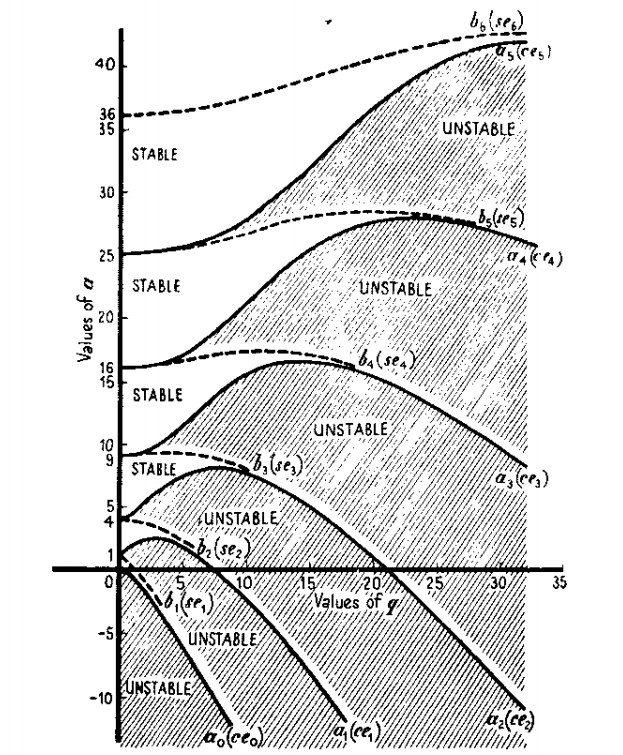
\includegraphics[width = 10cm]{Pictures/Mathieu_stability.PNG}
    \caption{Stability of solutions to Mathieu equation \eqref{eq:mathieu} taken from \cite{lachlan}.}
    \label{fig:mathieu_stability}
\end{figure}

\noindent
The solutions of the Mathieu equation are described in detail in \cite{lachlan}. For us, a~qualitative study will suffice. \Cref{fig:mathieu_stability} depicts the stability of solutions based on its parameters $a$ and $q$. We can see that if 

\begin{equation}
\label{eq:resonance}
    \lp \frac{2 k}{\omega \lambda} \rp^2 \approx n^2, \qquad n \in \Zbb
\end{equation}

\noindent
the string becomes unstable even for small amplitudes $A$. Physically, this corresponds to some kind of resonance between the natural frequency of the string $k$ (if there was no gravitational wave) and the frequency of the gravitational wave $\omega$. Also, if we fix the frequency $\omega$, the change of the amplitude $A$ will correspond to horizontal lines in \cref{fig:mathieu_stability}. On the other hand, fixing the amplitude $A$ to a~specific value and letting the frequency $\omega$ vary, will results in lines that intersect the origin with slope $2k^2/(A \lambda^2)$. Also, due to the inverse dependence on $\omega^2$, the higher the frequency, the closer we get to zero.

The same applies to the $y$ component, because the instability regions of the solutions of Mathieu equation are symmetric with respect to the sign of $q$. On the other hand, the $v$ component is more complicated and hard to interpret. Also, it would be hard to find a~good way to measure the energy of the string in this background, because the vector $\pardif{ }{\tau}$ can change from time-like to space-like during the motion. We will therefore turn to the next section, where we hope to solve this problem with different profile of gravitational waves.



%%%%%%%%%%%%%%%%%%%%%%%%% SECTION %%%%%%%%%%%%%%%%%%%%%%%%%%%%

\section{Gravitational wave burst with Gaussian profile}

In this section, we will study how a~burst of gravitational waves affects the motion of a~string in flat spacetime. We will choose $f(u)$ in \cref{eq:grav_H_polarisation_1} 
to be a cosine function multiplied by the a Gaussian envelope

\begin{equation}
\begin{aligned}
    H(u, x, y) &= (x^2 - y^2) \cos(\omega u) \exp \lp -\frac{(u-u_0)^2}{2 \rho^2} \rp \\
    &= (x^2 - y^2) \cos(\omega \lambda \tau) \exp \lp -\frac{\lambda^2(\tau-\tau_0)^2}{2 \rho^2} \rp
\end{aligned}
\end{equation}

\noindent
with frequency $\omega$ and the size of the Gaussian envelope $\rho$, which corresponds to the duration of the gravitational wave burst that hits its peak at proper time $\tau_0$. 

The string is initially in a~flat space, because $H$ is almost zero. Then comes the gravitational wave burst and after some time it fades away. During this time it is not easy to identify what is a~time-like coordinate and how the string really moves but after the burst ends, the metric returns again to the form of flat spacetime. This allows us to evaluate how the string changed its behaviour, specifically, to calculate the energy of the string before and after the gravitational wave burst hits it. We want to create a~graph showing the amount of energy transfered between the string and the gravitational wave burst and compare it with \cref{fig:mathieu_stability}. 

Calculation of the equations of motion from \cref{eq:EL} gives us


\begin{align}
    \begin{aligned}
        \difs[2]{v}{\tau} - \difs[2]{v}{\sigma} 
        - A \lambda \exp \lp -\frac{\lambda^2(\tau-\tau_0)^2}{2 \rho^2} \rp 
        \left[ \frac{ x^2 - y^2}{2} \omega \lambda \sin(\omega \lambda \tau) \right. \\
        \left. + \frac{ x^2 - y^2}{2} \frac{\lambda^2 (\tau - \tau_0)}{ \rho^2}\cos(\omega \lambda \tau)
        - 2 \lp x \difs[]{x}{\tau} - y \difs[]{y}{\tau} \rp \cos(\omega \lambda \tau) \right] = 0
        \end{aligned}        \\[3mm]
        \difs[2]{x}{\tau} - \difs[2]{x}{\sigma} - A \lambda^2 x \cos(\omega \lambda \tau)\exp \lp -\frac{\lambda^2(\tau-\tau_0)^2}{2 \rho^2} \rp & = 0 \\[3mm]
        \difs[2]{y}{\tau} - \difs[2]{y}{\sigma} + A \lambda^2 y \cos(\omega \lambda \tau)\exp \lp -\frac{\lambda^2(\tau-\tau_0)^2}{2 \rho^2} \rp & = 0
\end{align}

\noindent
Since $v$, $x$ and $y$ are $\sigma_1$ periodic in $\sigma$, we can expand them into Fourier series

\begin{align}
    v(\sigma, \tau) = \sum\limits_{k_v \in \Zbb} v_{k_v}(\tau) \me^{2 \pi \mi k_v \sigma/\sigma_1}
    \qquad & v_{k_v}(\tau) = \frac{1}{\sigma_1} \int\limits_{0}^{\sigma_1} v(\sigma, \tau) \me^{-2 \pi \mi k_v \sigma /\sigma_1} \\
    x(\sigma, \tau) = \sum\limits_{k_x \in \Zbb} x_{k_x}(\tau) \me^{2 \pi \mi k_x \sigma/\sigma_1}
    \qquad & x_{k_x}(\tau) = \frac{1}{\sigma_1} \int\limits_{0}^{\sigma_1} x(\sigma, \tau) \me^{-2 \pi \mi k_x \sigma /\sigma_1} \\
    y(\sigma, \tau) = \sum\limits_{k_y \in \Zbb} y_{k_y}(\tau) \me^{2 \pi \mi k_y \sigma/\sigma_1} 
    \qquad & y_{k_y}(\tau) = \frac{1}{\sigma_1} \int\limits_{0}^{\sigma_1} y(\sigma, \tau) \me^{-2 \pi \mi k_y \sigma /\sigma_1}
\end{align}

\noindent
The equations for $x$ and $y$ then take the form

\begin{align}
\label{eq:grav_x_expand}
\begin{aligned}
        \left[ \difs[2]{ }{\tau} - \difs[2]{ }{\sigma} - A \lambda^2 \cos(\omega \lambda \tau)\exp \lp -\frac{\lambda^2(\tau-\tau_0)^2}{2 \rho^2} \rp \right] \sum\limits_{k_x} x_{k_x} \me^{2 \pi \mi k_x \sigma /\sigma_1} \hspace{2cm}\\
        = \sum\limits_{k_x} \left[ \difs[2]{ }{\tau} + k_x^2 - A \lambda^2 \cos(\omega \lambda \tau)\exp \lp -\frac{\lambda^2(\tau-\tau_0)^2}{2 \rho^2} \rp \right] x_{k_x} \me^{2 \pi \mi k_x \sigma /\sigma_1} = 0
\end{aligned}
        \\[3mm]
\label{eq:grav_y_expand}
\begin{aligned}
        \left[ \difs[2]{ }{\tau} - \difs[2]{ }{\sigma} + A \lambda^2 \cos(\omega \lambda \tau)\exp \lp -\frac{\lambda^2(\tau-\tau_0)^2}{2 \rho^2} \rp \right] \sum\limits_{k_y} y_{k_y} \me^{2 \pi \mi k_y \sigma /\sigma_1}  \hspace{2cm}\\
        \sum\limits_{k_y} \left[ \difs[2]{ }{\tau} +k^2 + A \lambda^2 \cos(\omega \lambda \tau)\exp \lp -\frac{\lambda^2(\tau-\tau_0)^2}{2 \rho^2} \rp \right]  y_{k_y} \me^{2 \pi \mi k_y \sigma /\sigma_1} = 0
\end{aligned}
 \end{align}
 
\noindent
In order for this to be equal to zero, every term in the sum must vanish. The equation for $v$ is a little bit more complicated, so for more clear view of the equations, we will denote

\begin{align}
    h(\tau) &  = \frac{A \lambda}{2} \exp \lp -\frac{\lambda^2(\tau-\tau_0)^2}{2 \rho^2} \rp \left[ \omega \lambda \sin(\omega \lambda \tau) + \frac{\lambda^2 (\tau - \tau_0)}{ \rho^2}\cos(\omega \lambda \tau) \right] \\
    b(\tau) & = 2 A \lambda \exp \lp -\frac{\lambda^2(\tau-\tau_0)^2}{2 \rho^2} \rp \cos(\omega \lambda \tau)
\end{align}

\noindent
If we multiply the equation by $\me^{-2 \pi \mi k_v \sigma / \sigma_1}$ and integrate over $\sigma$, we get

\begin{equation}
\label{eq:grav_v_expand}
\begin{aligned}
    \int\limits_{0}^{\sigma_1} \me^{-2 \pi \mi k_v \sigma /\sigma_1} \lp \difs[2]{ }{\tau} - \difs[2]{ }{\sigma} \rp v \D \sigma = \hspace{6cm} \\
    = \int\limits_{0}^{\sigma_1} \me^{-2 \pi \mi k_v \sigma /\sigma_1} 
    \left[ \lp x^2-y^2 \rp h(\tau) - \lp x \, \difs[]{x}{\tau} - y \, \difs[]{y}{\tau} \rp b(\tau) \right] \D \sigma
\end{aligned}
\end{equation}

\noindent
We will modify each side of the equation independently. The left side can be written as

\begin{equation}
\label{eq:grav_v_expand_left}
\begin{aligned}
    \int\limits_{0}^{\sigma_1} \me^{-2 \pi \mi k_v \sigma /\sigma_1} \lp \difs[2]{ }{\tau} - \difs[2]{ }{\sigma} \rp \sum\limits_{k_v'} v_{k_v'} \me^{\mi k_v' \sigma} \D \sigma
    &= \sum\limits_{k_v'} \int\limits_{0}^{\sigma_1} \me^{-2 \pi \mi \lp k_v - k_v' \rp \sigma /\sigma_1} \D \sigma \lp \difs[2]{ }{\tau} + {k_v'}^2  \rp v_{k_v'} \\[3mm]
    = \sum\limits_{k_v'} \sigma_1 \delta^{k_v'}_{k_v} \lp \difs[2]{ }{\tau} + {k_v'}^2  \rp v_{k_v'} 
    &= \sigma_1 \lp \difs[2]{ }{\tau} + {k_v}^2  \rp v_{k_v}
\end{aligned}
\end{equation}

\noindent
Simplifying the first term on the right side of \cref{eq:grav_v_expand} gives us

\begin{equation}
\label{eq:grav_v_expand_right1}
\begin{aligned}
    \int\limits_{0}^{\sigma_1} \me^{-2 \pi \mi k_v \sigma /\sigma_1} 
    \lp \sum\limits_{k_x} \sum\limits_{k_x'} x_{k_x} x_{k_x'} \me^{2 \pi\mi (k_x + k_x') \sigma /\sigma_1}
    - \sum\limits_{k_y} \sum\limits_{k_y'} y_{k_y} y_{k_y'} \me^{2 \pi\mi (k_y + k_y') \sigma /\sigma_1} \rp 
    h(\tau) \D \sigma \\
    = \lp \sum\limits_{k_x k_x'} x_{k_x} x_{k_x'} \int\limits_{0}^{\sigma_1} \me^{2 \pi \mi (k_x + k_x' - k_v) \sigma /\sigma_1} \D \sigma
    - \sum\limits_{k_y k_y'} y_{k_y} y_{k_y'} \int\limits_{0}^{\sigma_1} \me^{2 \pi \mi (k_y + k_y' - k_v) \sigma /\sigma_1} \D \sigma \rp 
    h(\tau) \\
    = \sigma_1 \lp \sum\limits_{k_x k_x'} x_{k_x} x_{k_x'} \delta^{k_x'}_{k_v - k_x}
    - \sum\limits_{k_y k_y'} y_{k_y} y_{k_y'} \delta^{k_y'}_{k_v - k_y} \rp 
    h(\tau) \\
    = \sigma_1 \lp \sum\limits_{k_x} x_{k_x} x_{k_v - k_x} - \sum\limits_{k_y} y_{k_y} y_{k_v - k_y} \rp h(\tau)
\end{aligned}
\end{equation}

\noindent
The second term on the right side of \cref{eq:grav_v_expand} will end up similarly to the first term

\begin{equation}
\label{eq:grav_v_expand_right2}
\begin{aligned}
	\int\limits_{0}^{\sigma_1} \me^{-2 \pi \mi k_v \sigma /\sigma_1} 
    \lp \sum\limits_{k_x k_x'} x_{k_x} \difs[]{x_{k_x'}}{\tau} \me^{2 \pi\mi (k_x + k_x') \sigma /\sigma_1}
    - \sum\limits_{k_y k_y'} y_{k_y} \difs[]{y_{k_y'}}{\tau} \me^{2 \pi\mi (k_y + k_y') \sigma /\sigma_1} \rp 
    b(\tau) \D \sigma \\
    = \sigma_1 \lp \sum\limits_{k_x k_x'} x_{k_x} \difs[]{x_{k_x'}}{\tau} \delta^{k_x'}_{k_v - k_x}
    - \sum\limits_{k_y k_y'} y_{k_y} \difs[]{y_{k_y'}}{\tau} \delta^{k_y'}_{k_v - k_y} \rp 
    b(\tau) \\
    = \sigma_1 \lp \sum\limits_{k_x} x_{k_x} \difs[]{x_{k_v - k_x}}{\tau} 
    - \sum\limits_{k_y} y_{k_y} \difs[]{y_{k_v - k_y}}{\tau} \rp b(\tau)
\end{aligned}
\end{equation}


\noindent
Combining \cref{eq:grav_v_expand_left} with \cref{eq:grav_v_expand_right1} and \cref{eq:grav_v_expand_right2}, we arrive at equation for $v_{k_v}$

\begin{equation}
\label{eq:grav_v_expand_fin}
\begin{aligned}
    \lp \difs[2]{ }{\tau} + {k_v}^2  \rp v_{k_v} = 
    \lp \sum\limits_{k_x} x_{k_x} x_{k_v - k_x} h(\tau) 
    - x_{k_x} \difs[]{x_{k_v - k_x}}{\tau} b(\tau) \right. \\
    \left. + \sum\limits_{k_y} y_{k_y} \difs[]{y_{k_v - k_y} b(\tau)}{\tau} 
    - y_{k_y} y_{k_v - k_y} h(\tau) \rp
\end{aligned}
\end{equation}

\noindent
\Cref{eq:grav_x_expand,eq:grav_y_expand,eq:grav_v_expand_fin} together with \cref{eq:grav_u} describe the motion of the string affected by the gravitational wave burst. We can notice, that the equations for $x_{k_x}$ \eqref{eq:grav_x_expand} and $y_{k_y}$ \eqref{eq:grav_y_expand} depend only on the $k_x$ or $k_y$ modes respectively. Therefore, we can say that every mode that is zero at the beginning will also be zero throughout the motion. However, the $k_v$-th mode of $v$ is affected by the modes of $x$ and $y$.

We will study a~string that is initially circular in the $x$, $y$ plane. The components $x_{k_x}$ and $y_{k_y}$ are nonzero only for $k_{x/y} = \pm 1$, specifically

\begin{equation}
\begin{aligned}
    x_1 = \frac{r_0}{2},& \qquad x_{-1} = \frac{r_0}{2} \\
    y_1 = \frac{r_0}{2 \mi},& \qquad y_{-1} = -\frac{r_0}{2 \mi}
\end{aligned}
\end{equation}

\noindent
Furthermore, we will set the $k_v = 0$ mode to be $v_0 = \varepsilon \tau$. The contributions from the $x$ and $y$ modes will affect only $k_v = \{ -2, 0, 2\}$ modes. We want to look at a~string that is initially in rest with respect to the observer and is in static gauge. This can be satisfied if

\begin{align}
    \difs[]{t}{\tau}(\tau = 0) = \difs[]{\frac{\sqrt{2}(u-v)}{2}}{\tau} = \frac{\sqrt{2}(\lambda - \varepsilon)}{2} = 1 \\
    \difs[]{z}{\tau}(\tau = 0) = \difs[]{\frac{\sqrt{2}(u+v)}{2}}{\tau} = \frac{\sqrt{2}(\lambda + \varepsilon)}{2} = 0
\end{align}

\noindent
This gives us the initial parameterization of the string

\begin{equation}
    \lambda = -\varepsilon = \frac{1}{\sqrt{2}}
\end{equation}

\noindent
Now we can solve the \cref{eq:grav_x_expand,eq:grav_y_expand,eq:grav_v_expand_fin} numerically with these initial values. Since the behaviour of the strings varies a~lot, we will measure the rest energy of the string after its interaction with the gravitational wave burst. This energy is given by \cref{eq:flat_rest_energy}. After the gravitational wave burst has passed, the spacetime is flat again. We can therefore make the same arguments as in \cref{sec:rest_energy} and arrive at the fact that the only contribution to the four-momenta will come from the $0$-th modes. The only non-zero components of the four-momenta are given by

\begin{align}
    p_u = \int\limits_0^{\sigma_1} \difs[]{v}{\tau} \D \sigma = \phi \sigma_1 \\
    p_v = \int\limits_0^{\sigma_1} \difs[]{u}{\tau} \D \sigma = \lambda \sigma_1
\end{align}

\noindent
where we denoted the part of $v$ that is proportional to $\tau$ as $\phi$. This follows from the fact, that only $0$-th $k_v$ mode is not zero when integrated over $\{0, 2 \pi\}$ and the constant term vanishes with the $\tau$ derivative. The rest energy of the string is then calculated as

\begin{equation}
    m = \sigma_1 \sqrt{-2 \lambda \difs[]{v}{\tau}}
\end{equation}

\noindent
We performed a series of numerical solutions of \cref{eq:grav_v_expand_fin} while varying the parameters of frequency $\omega$ and amplitude $A$ of the gravitational wave. Furthermore, we calculated the energy before and after the gravitational wave burst and plotted their fraction $E/E_0$ in \cref{fig:grav_energy} and \cref{fig:grav_energy_small}. Note, that we chose the logarithmic scale for $E/E_0$, because otherwise, only very bright spots would be visible in the whole graph. In this figure, we can see, that there are some resonance frequencies for which the energy recieved by the string is high even for small amplitudes of the gravitational wave. In fact, these resonant frequencies perfectly correspond with \cref{fig:mathieu_stability} and \cref{eq:resonance}, where we have regions of instability of the solutions. We chose $k = 1$ and $\lambda = 1/\sqrt{2}$. Therefore for frequencies 

\begin{equation}
	\omega \approx \frac{2 \sqrt{2}}{n}, \qquad n \in \Zbb
\end{equation}

\noindent
the interaction of gravitational wave with the string affects the string much more than for other frequencies even if it has small amplitude. The rest energy is not the only thing the string acquires from the gravitational wave. The string also gets pushed in the direction of the propagation of the gravitational wave $z$. The velocity of the centre of mass of the string in the $j$ spatial direction is given by

\begin{equation}
	v^j = \frac{p^j}{p^t}
\end{equation}

\noindent
The velocity in the $z$ direction is plotted for various frequencies $\omega$ and amplitudes $A$ of the gravitational wave in \cref{fig:grav_velocity} \cref{fig:grav_velocity_small}. All in all, the string can receive or loose both rest energy and velocity in the direction of the propagation of the gravitational wave during the interaction with the gravitational wave. But for some resonant frequencies, the effect of the gravitational wave is of few orders higher, than the rest.

Also, because we want the reader to get a notion of how the evolution of the string looks like, we add two plots of the motion of the string. One for a resonant frequency in \cref{fig:grav_evol_res} and one for non-resonant frequency in \cref{fig:grav_evol_nonres}.

\begin{figure}[p]
    \centering
    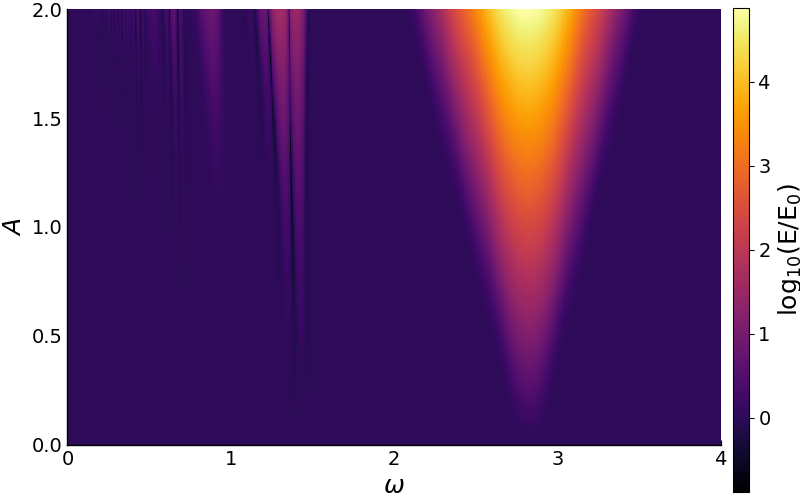
\includegraphics[width=1.0 \textwidth]{pictures/grav_energy.png}
    \caption{Rest energy received or taken away by the gravitational wave burst based on its frequency and amplitude.}
    \label{fig:grav_energy}
\end{figure}

\begin{figure}[p]
	\centering
	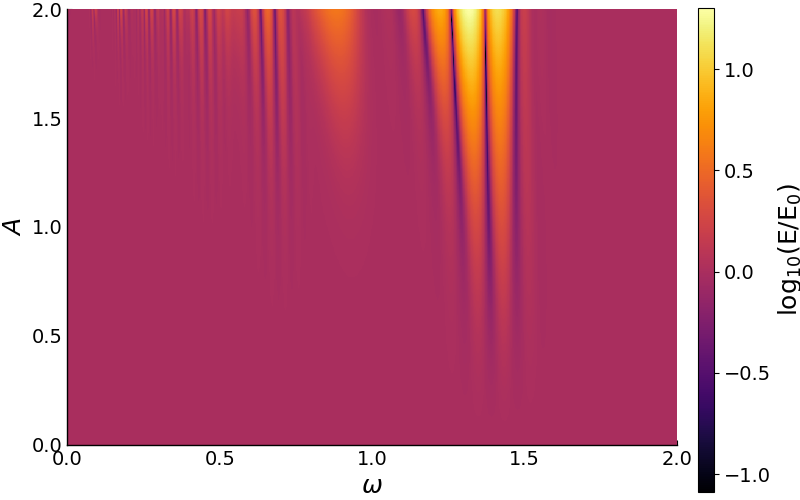
\includegraphics[width=1.0 \textwidth]{pictures/grav_energy_small.png}
	\caption{Energy received or taken away by the gravitational wave burst based on its frequency and amplitude with detail on smaller frequencies.}
	\label{fig:grav_energy_small}
\end{figure}


\begin{figure}[p]
	\centering
	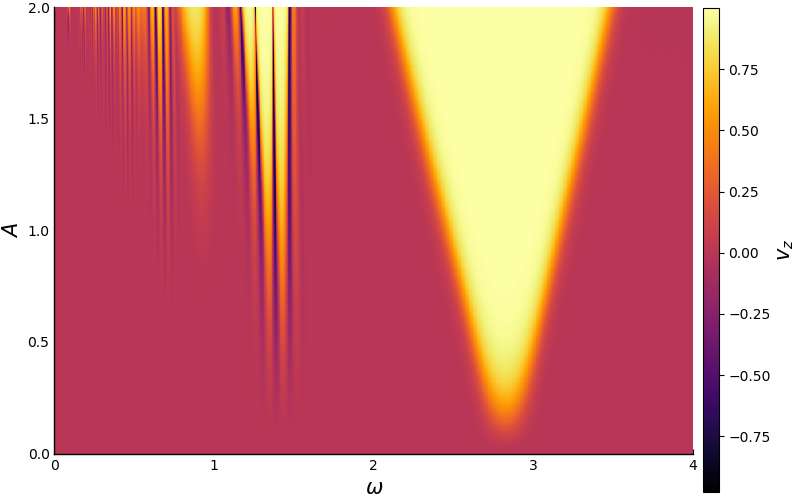
\includegraphics[width=1.0 \textwidth]{pictures/grav_velocity.png}
	\caption{Velocity of the string in $z$ direction after the gravitational wave burst with frequency $\omega$ and amplitude $A$.}
	\label{fig:grav_velocity}
\end{figure}


\begin{figure}[p]
	\centering
	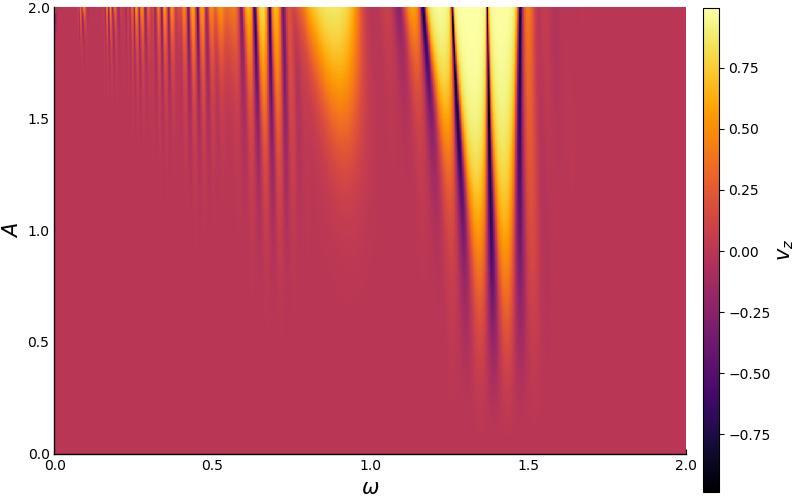
\includegraphics[width=1.0 \textwidth]{pictures/grav_velocity_small.png}
	\caption{Velocity of the string in $z$ direction after the gravitational wave burst with frequency $\omega$ and amplitude $A$ with detail on smaller frequencies.}
	\label{fig:grav_velocity_small}
\end{figure}

\begin{figure}[p]
	\centering
	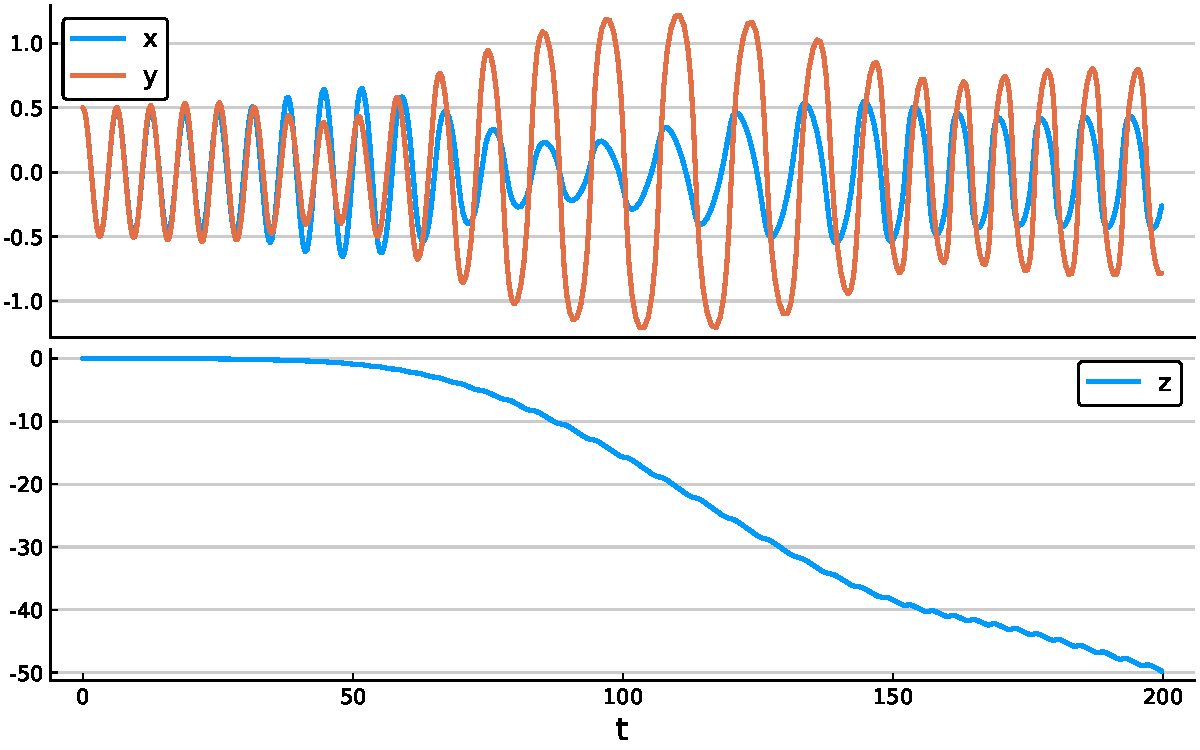
\includegraphics[width=1.0 \textwidth]{pictures/grav_evol_res.pdf}
	\caption{The evolution of a string while interacting with the gravitational wave burst, that has resonant frequency $\omega = 2 \sqrt{2} - 0.2$ and amplitude $A = 0.5$.}
	\label{fig:grav_evol_res}
\end{figure}

\begin{figure}[p]
	\centering
	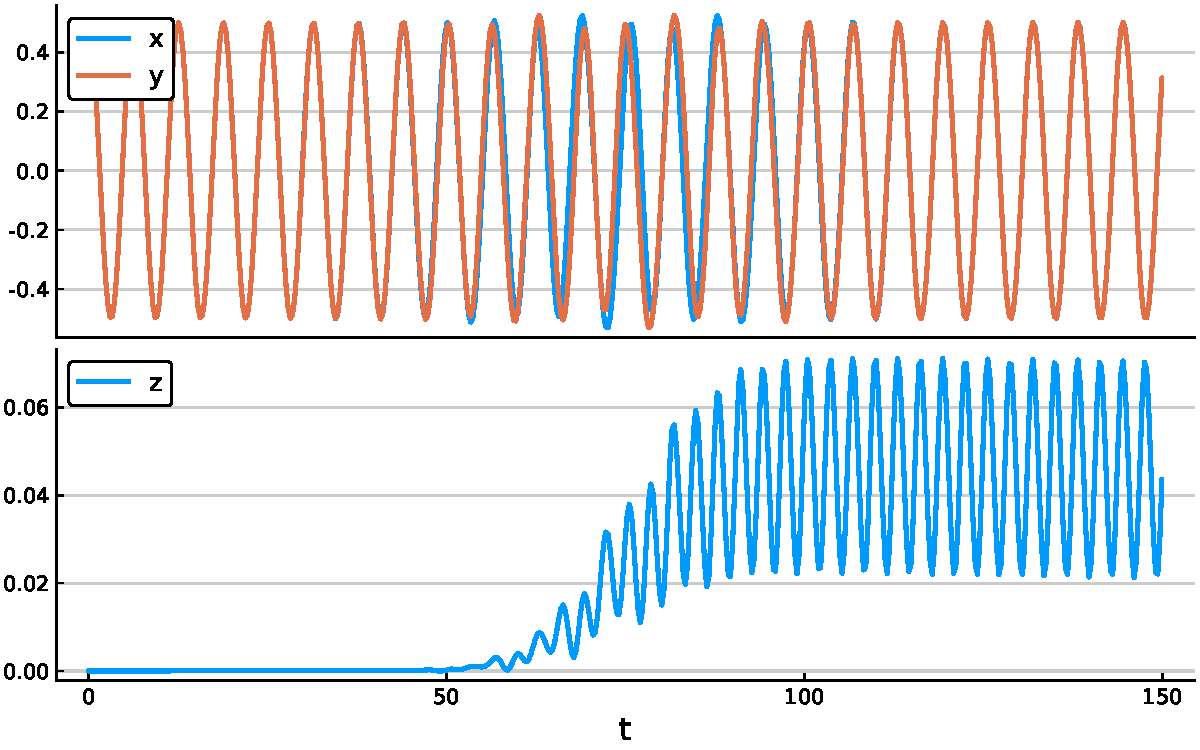
\includegraphics[width=1.0 \textwidth]{pictures/grav_evol_nonres.pdf}
	\caption{The evolution of a string while interacting with the gravitational wave burst, that has non-resonant frequency $\omega = 0.5$ and amplitude $A = 0.5$.}
	\label{fig:grav_evol_nonres}
\end{figure}



